\documentclass[aspectratio=1610]{beamer}

\usepackage{tikz}
\usepackage{minted}
\usepackage{bbding}

\newcommand{\correctans}{\textcolor{green!50!black}{\CheckmarkBold}}
\newcommand{\wrongans}{\textcolor{red!50!black}{\XSolidBold}}

% The following were provided by Inkscape:
\definecolor{cDCDEE0}{RGB}{220,222,224}
\definecolor{c85888D}{RGB}{133,136,141}
\definecolor{c70BF41}{RGB}{112,191,65}
\definecolor{cC82506}{RGB}{200,37,6}
\definecolor{c45BEEE}{RGB}{69,190,238}
\definecolor{c009CFD}{RGB}{0,156,253}
\definecolor{cFFFFFF}{RGB}{255,255,255}
\definecolor{cB5B5B5}{RGB}{181,181,181}
\definecolor{c231F20}{RGB}{35,31,32}
\definecolor{cB285BC}{RGB}{178,133,188}
\definecolor{c45beee}{RGB}{69,190,238}

\usetikzlibrary{tikzmark}

\begin{document}

\begin{frame}
\title{Version Control with Git}
\date{March 2017, Winona State University}

\maketitle

\end{frame}

\begin{frame}

\begin{itemize}
  \item Lesson plan taken from Software Carpentry: \url{http://swcarpentry.github.io/git-novice/}
  \item This presentation is on GitHub:
  \url{https://github.com/christopherphan/Winona-SC-git}
\end{itemize}

\end{frame}

\begin{frame}
  \frametitle{Motivating example\footnote{\url{http://swcarpentry.github.io/git-novice/}}}
\begin{itemize}
\item  Wolfman and Dracula have been hired to investigate if it is possible to send a planetary lander to Mars. \pause
\item Want to be able to work on the plans at the same time.\pause
\item Two aproaches: \pause
\begin{itemize} \item Take turns. \pause \textcolor{red!50!black}{\textbf{Problem}: Each one will spend a lot of time waiting for the other to finish.} \pause
  \item Work on their own copies and email changes back and forth. \pause \textcolor{red!50!black}{\textbf{Problem}: Things will be lost, overwritten, or duplicated.}
\end{itemize}
\end{itemize}
\end{frame}


\begin{frame}
  \frametitle{How it works\footnote{\url{http://swcarpentry.github.io/git-novice/01-basics/}}}
\resizebox{0.8\textwidth}{!}{
\begin{minipage}{\textwidth}
  % This was converted from
  % <http://swcarpentry.github.io/git-novice/fig/play-changes.svg> using
  % Inkscape
  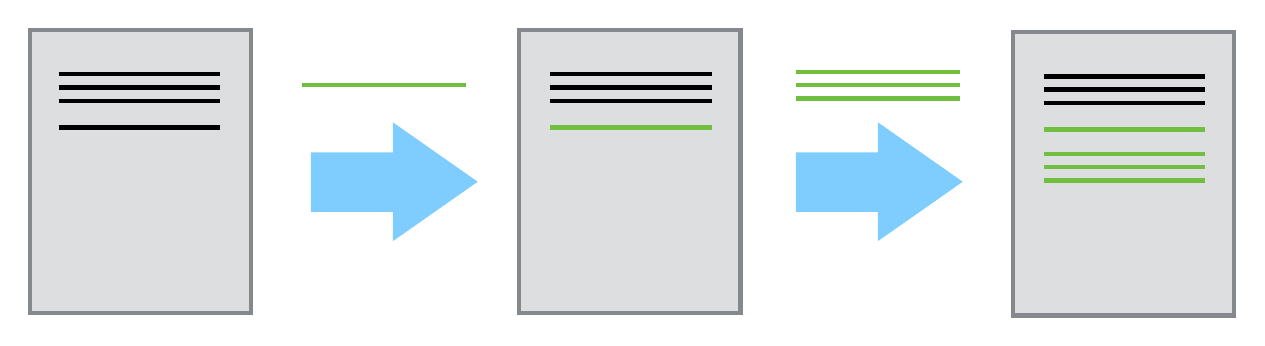
\begin{tikzpicture}[y=0.80pt,x=0.80pt,yscale=-1, inner sep=0pt, outer sep=0pt]
      \path[fill=cDCDEE0,rounded corners=0.0000cm] (37.0000,30.0000) rectangle
        (137.0000,158.0000);
      \path[draw=c85888D,line width=1.600pt,rounded corners=0.0000cm]
        (37.0000,30.0000) rectangle (137.0000,158.0000);
      \path[draw=black,line width=1.600pt] (50.0000,50.0000) -- (123.0000,50.0000);
      \path[draw=black,line width=1.600pt] (50.0000,56.0000) -- (123.0000,56.0000);
      \path[draw=black,line width=1.600pt] (50.0000,62.0000) -- (123.0000,62.0000);
      \path[draw=black,line width=1.600pt] (50.0000,74.0000) -- (123.0000,74.0000);
      \path[fill=cDCDEE0,rounded corners=0.0000cm] (258.0000,30.0000) rectangle
        (358.0000,158.0000);
      \path[draw=c85888D,line width=1.600pt,rounded corners=0.0000cm]
        (258.0000,30.0000) rectangle (358.0000,158.0000);
      \path[draw=black,line width=1.600pt] (272.0000,50.0000) -- (345.0000,50.0000);
      \path[draw=black,line width=1.600pt] (272.0000,56.0000) -- (345.0000,56.0000);
      \path[draw=black,line width=1.600pt] (272.0000,62.0000) -- (345.0000,62.0000);
      \path[draw=c70BF41,line width=1.600pt] (272.0000,74.0000) -- (345.0000,74.0000);
      \path[draw=c70BF41,line width=1.600pt] (160.0000,55.0000) -- (234.0000,55.0000);
      \path[fill=cDCDEE0,rounded corners=0.0000cm] (481.0000,31.0000) rectangle
        (581.0000,159.0000);
      \path[draw=c85888D,line width=1.600pt,rounded corners=0.0000cm]
        (481.0000,31.0000) rectangle (581.0000,159.0000);
      \path[draw=black,line width=1.600pt] (495.0000,51.0000) -- (568.0000,51.0000);
      \path[draw=black,line width=1.600pt] (495.0000,57.0000) -- (568.0000,57.0000);
      \path[draw=black,line width=1.600pt] (495.0000,63.0000) -- (568.0000,63.0000);
      \path[draw=c70BF41,line width=1.600pt] (495.0000,75.0000) -- (568.0000,75.0000);
      \path[draw=c70BF41,line width=1.600pt] (495.0000,86.0000) -- (568.0000,86.0000);
      \path[draw=c70BF41,line width=1.600pt] (495.0000,92.0000) -- (568.0000,92.0000);
      \path[draw=c70BF41,line width=1.600pt] (495.0000,98.0000) -- (568.0000,98.0000);
      \path[draw=c70BF41,line width=1.600pt] (383.0000,49.0000) -- (457.0000,49.0000);
      \path[draw=c70BF41,line width=1.600pt] (383.0000,55.0000) -- (457.0000,55.0000);
      \path[draw=c70BF41,line width=1.600pt] (383.0000,61.0000) -- (457.0000,61.0000);
    \begin{scope}[opacity=0.500,transparency group]
      \path[fill=c009CFD,rounded corners=0.0000cm] (163.9310,85.2760) rectangle
        (208.7960,112.1950);
        \path[fill=c009CFD] (200.9410,125.4290) -- (239.2750,98.5880) --
          (200.9410,71.7430) -- cycle;
    \end{scope}
    \begin{scope}[opacity=0.500,transparency group]
      \path[fill=c009CFD,rounded corners=0.0000cm] (383.0160,85.2760) rectangle
        (427.8810,112.1950);
        \path[fill=c009CFD] (420.0260,125.4290) -- (458.3590,98.5880) --
          (420.0260,71.7430) -- cycle;
    \end{scope}

  \end{tikzpicture}

\end{minipage}
}
\pause
\vskip 1 em
``Unlimted undo!''

\end{frame}

\begin{frame}
\frametitle{Why version control?}

\begin{quote}[M]otivating git: You mostly collaborate with yourself, and me-from-two-months-ago never responds to email.---Karen Cranston\footnote{\url{http://bit.ly/motivate_git}}
\end{quote}

\pause

\vskip 2 em


\begin{quote}
  [Y]ou can now freely throw away bits and pieces, secure in the knowledge that if you actually want them back, they are there in the revision control system. Interestingly, almost nobody actually uses this feature. Revision control systems are not there to save your old work. They are there to give you permission to throw that old work away.\\
  ---Peter Boothe\footnote{Quoted at \url{http://tex.stackexchange.com/a/1135/52}}
\end{quote}

\end{frame}

\begin{frame}
  \frametitle{How it works\footnote{\url{http://swcarpentry.github.io/git-novice/01-basics/}}}

  \resizebox{0.4\textwidth}{!}{
  \begin{minipage}{\textwidth}
    % This was converted from
    % <http://swcarpentry.github.io/git-novice/fig/versions.svg> using
    % Inkscape
    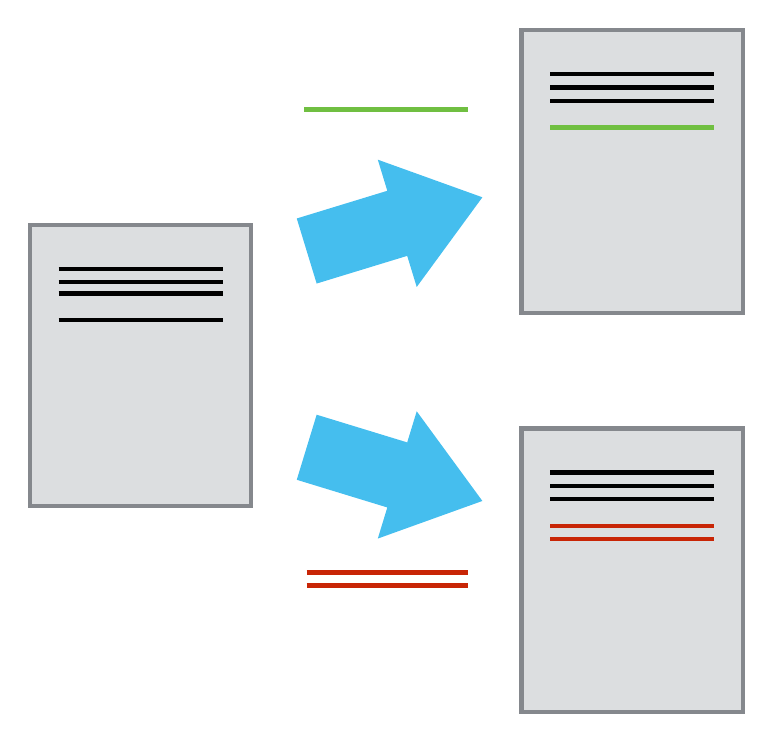
\begin{tikzpicture}[y=0.80pt,x=0.80pt,yscale=-1, inner sep=0pt, outer sep=0pt]
      \path[fill=cDCDEE0,rounded corners=0.0000cm] (33.0000,111.0000) rectangle
        (133.0000,238.0000);
      \path[draw=c85888D,line width=1.600pt,rounded corners=0.0000cm]
        (33.0000,111.0000) rectangle (133.0000,238.0000);
      \path[draw=black,line width=1.600pt] (46.0000,131.0000) -- (120.0000,131.0000);
      \path[draw=black,line width=1.600pt] (46.0000,137.0000) -- (120.0000,137.0000);
      \path[draw=black,line width=1.600pt] (46.0000,142.0000) -- (120.0000,142.0000);
      \path[draw=black,line width=1.600pt] (46.0000,154.0000) -- (120.0000,154.0000);
      \path[fill=cDCDEE0,rounded corners=0.0000cm] (255.0000,23.0000) rectangle
        (355.0000,151.0000);
      \path[draw=c85888D,line width=1.600pt,rounded corners=0.0000cm]
        (255.0000,23.0000) rectangle (355.0000,151.0000);
      \path[draw=black,line width=1.600pt] (268.0000,43.0000) -- (342.0000,43.0000);
      \path[draw=black,line width=1.600pt] (268.0000,49.0000) -- (342.0000,49.0000);
      \path[draw=black,line width=1.600pt] (268.0000,55.0000) -- (342.0000,55.0000);
      \path[draw=c70BF41,line width=1.600pt] (268.0000,67.0000) -- (342.0000,67.0000);
      \path[draw=c70BF41,line width=1.600pt] (157.0000,59.0000) -- (231.0000,59.0000);
    \path[fill=c45BEEE] (203.4270,125.0670) -- (207.7240,139.1220) --
      (237.3820,98.6160) -- (190.1440,81.6200) -- (194.4400,95.6750) --
      (153.5410,108.1790) -- (162.5270,137.5710) -- cycle;
      \path[fill=cDCDEE0,rounded corners=0.0000cm] (255.0000,203.0000) rectangle
        (355.0000,331.0000);
      \path[draw=c85888D,line width=1.600pt,rounded corners=0.0000cm]
        (255.0000,203.0000) rectangle (355.0000,331.0000);
      \path[draw=black,line width=1.600pt] (268.0000,223.0000) -- (342.0000,223.0000);
      \path[draw=black,line width=1.600pt] (268.0000,229.0000) -- (342.0000,229.0000);
      \path[draw=black,line width=1.600pt] (268.0000,235.0000) -- (342.0000,235.0000);
      \path[draw=cC82506,line width=1.600pt] (268.0000,247.0000) --
        (342.0000,247.0000);
    \path[fill=c45BEEE] (194.4400,238.7130) -- (190.1440,252.7670) --
      (237.3820,235.7710) -- (207.7240,195.2660) -- (203.4270,209.3200) --
      (162.5270,196.8150) -- (153.5410,226.2080) -- cycle;
      \path[draw=cC82506,line width=1.600pt] (268.0000,253.0000) --
        (342.0000,253.0000);
      \path[draw=cC82506,line width=1.600pt] (158.0000,268.0000) --
        (231.0000,268.0000);
      \path[draw=cC82506,line width=1.600pt] (158.0000,274.0000) --
        (231.0000,274.0000);

    \end{tikzpicture}
  \end{minipage}
} \hfill \pause
\resizebox{0.4\textwidth}{!}{
\begin{minipage}{\textwidth}
  % This was converted from
  % <http://swcarpentry.github.io/git-novice/fig/merge.svg> using
  % Inkscape
  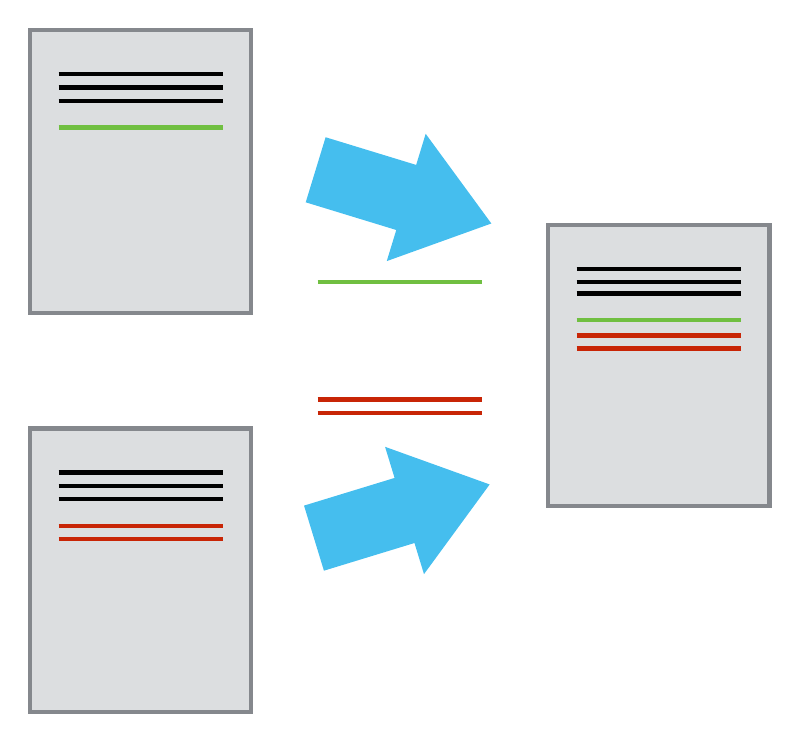
\begin{tikzpicture}[y=0.80pt,x=0.80pt,yscale=-1, inner sep=0pt, outer sep=0pt]
    \path[fill=cDCDEE0,rounded corners=0.0000cm] (266.0000,129.0000) rectangle
      (366.0000,256.0000);
    \path[draw=c85888D,line width=1.600pt,rounded corners=0.0000cm]
      (266.0000,129.0000) rectangle (366.0000,256.0000);
    \path[draw=black,line width=1.600pt] (279.0000,149.0000) -- (353.0000,149.0000);
    \path[draw=black,line width=1.600pt] (279.0000,155.0000) -- (353.0000,155.0000);
    \path[draw=black,line width=1.600pt] (279.0000,160.0000) -- (353.0000,160.0000);
    \path[draw=c70BF41,line width=1.600pt] (279.0000,172.0000) --
      (353.0000,172.0000);
    \path[fill=cDCDEE0,rounded corners=0.0000cm] (32.0000,41.0000) rectangle
      (132.0000,169.0000);
    \path[draw=c85888D,line width=1.600pt,rounded corners=0.0000cm]
      (32.0000,41.0000) rectangle (132.0000,169.0000);
    \path[draw=black,line width=1.600pt] (45.0000,61.0000) -- (119.0000,61.0000);
    \path[draw=black,line width=1.600pt] (45.0000,67.0000) -- (119.0000,67.0000);
    \path[draw=black,line width=1.600pt] (45.0000,73.0000) -- (119.0000,73.0000);
    \path[draw=c70BF41,line width=1.600pt] (45.0000,85.0000) -- (119.0000,85.0000);
    \path[draw=c70BF41,line width=1.600pt] (162.0000,155.0000) --
      (236.0000,155.0000);
    \path[fill=cDCDEE0,rounded corners=0.0000cm] (32.0000,221.0000) rectangle
      (132.0000,349.0000);
    \path[draw=c85888D,line width=1.600pt,rounded corners=0.0000cm]
      (32.0000,221.0000) rectangle (132.0000,349.0000);
    \path[draw=black,line width=1.600pt] (45.0000,241.0000) -- (119.0000,241.0000);
    \path[draw=black,line width=1.600pt] (45.0000,247.0000) -- (119.0000,247.0000);
    \path[draw=black,line width=1.600pt] (45.0000,253.0000) -- (119.0000,253.0000);
    \path[draw=cC82506,line width=1.600pt] (45.0000,265.0000) --
      (119.0000,265.0000);
  \path[fill=c45BEEE] (205.7110,272.7680) -- (210.0080,286.8220) --
    (239.6660,246.3160) -- (192.4280,229.3200) -- (196.7250,243.3750) --
    (155.8250,255.8790) -- (164.8120,285.2710) -- cycle;
  \path[fill=c45BEEE] (197.4880,131.3840) -- (193.1910,145.4380) --
    (240.4300,128.4430) -- (210.7710,87.9370) -- (206.4750,101.9920) --
    (165.5740,89.4870) -- (156.5880,118.8800) -- cycle;
    \path[draw=cC82506,line width=1.600pt] (45.0000,271.0000) --
      (119.0000,271.0000);
    \path[draw=cC82506,line width=1.600pt] (162.0000,208.0000) --
      (236.0000,208.0000);
    \path[draw=cC82506,line width=1.600pt] (162.0000,214.0000) --
      (236.0000,214.0000);
    \path[draw=cC82506,line width=1.600pt] (279.0000,179.0000) --
      (353.0000,179.0000);
    \path[draw=cC82506,line width=1.600pt] (279.0000,185.0000) --
      (353.0000,185.0000);

  \end{tikzpicture}
\end{minipage}
}
\pause

Different people can operate on the same file simultaneously.

\end{frame}

\begin{frame}[fragile]
\frametitle{Set-up\footnote{\url{http://swcarpentry.github.io/git-novice/02-setup/}}}

\textcolor{red!50!black}{Don't type the \texttt{\$}s!}

\vskip 1 em

Configure git (replace the name and email address with your own)
\begin{minted}{shell}
$ git config --global user.name "Vlad Dracula"
$ git config --global user.email "vlad@tran.sylvan.ia"
$ git config --global color.ui "auto"
$ git config --global core.editor "nano -w"
\end{minted}

\pause

Check all settings:
\begin{minted}{shell}
$ git config --list
\end{minted}

\vskip 1 em
\pause

Can always get help, e.g.:
\begin{minted}{shell}
$ git config -h
$ git config --help
\end{minted}

\vskip 1 em
Or can consult: \textit{Pro Git}, by Scott Chacon and Ben Straub, available for free at: \url{https://git-scm.com/book/en/v2}

\end{frame}

\begin{frame}[fragile]
\frametitle{Creating a repository\footnote{http://swcarpentry.github.io/git-novice/03-create/}}

\textcolor{red!50!black}{Don't type the \texttt{\$}s!}

Create a directory:
\begin{minted}{shell}
$ mkdir planets
$ cd planets
\end{minted}

\pause
Turn it into a git repository:
\begin{minted}{shell}
$ git init
\end{minted}
\pause

See that a new folder called \mintinline{shell}{.git} has been created.
\begin{minted}{shell}
$ ls -a
\end{minted}
\pause

Check the status of our repository:
\begin{minted}{shell}
$ git status
\end{minted}

\end{frame}

\begin{frame}[fragile]
  \frametitle{Tracking changes\footnote{http://swcarpentry.github.io/git-novice/04-changes/}}

  Create a file called \texttt{mars.txt} (e.g.~using \texttt{nano}) with the following content:

\begin{minted}{text}
Cold and dry, but everything is my favorite color
\end{minted}

  \pause

\vskip 1 em

Verify the file exists and its contents:

\begin{minted}{shell}
$ ls
$ cat mars.txt
\end{minted}

\pause

\vskip 1 em

Check the status of our repo:
\begin{minted}{shell}
$ git status
\end{minted}

\vskip 1 em
\pause

Add the file to our repo:
\begin{minted}{shell}
$ git add mars.txt
$ git status
\end{minted}

\vskip 1 em
\pause


\end{frame}

\begin{frame}[fragile]
  \frametitle{Tracking changes\footnote{http://swcarpentry.github.io/git-novice/04-changes/}}

  Commit to our repo:
  \begin{minted}{shell}
$ git commit -m "Start notes on Mars as a base"
$ git status
  \end{minted}

  \pause
  \vskip 1 em

Verify in the log:
\begin{minted}{shell}
$ git log
\end{minted}

\vskip 1 em

\pause

Edit the file \texttt{mars.txt} so that it reads (e.g.~using \texttt{nano}):
\begin{minted}{text}
Cold and dry, but everything is my favorite color
The two moons may be a problem for Wolfman
\end{minted}
\pause

\vskip 1 em

Recheck the status:
\begin{minted}{shell}
$ git status
\end{minted}

\end{frame}

\begin{frame}[fragile]
  \frametitle{Tracking changes\footnote{http://swcarpentry.github.io/git-novice/04-changes/}}

See difference between the current folder contents and repo:
\begin{minted}{shell}
$ git diff
\end{minted}
\vskip 1 em
\pause

Now, commit the new changes to your repo:
\begin{minted}{shell}
$ git commit -m "Add concerns about effects of Mars' moons on Wolfman"
$ git status
\end{minted}
\vskip 1 em
\pause

\textcolor{red!50!black}{This didn't work, because we have to add first:}
\begin{minted}{shell}
$ git add mars.txt
$ git commit -m "Add concerns about effects of Mars' moons on Wolfman"
$ git status
\end{minted}


\end{frame}


\begin{frame}[fragile]
\frametitle{Exercise: Committing Changes to Git\footnote{\url{http://swcarpentry.github.io/git-novice/04-changes/\#committing-changes-to-git}}}

Which command(s) below would save the changes of \texttt{myfile.txt} to my local Git repository?
\begin{enumerate}
\item \begin{minted}{shell}
$ git commit -m "my recent changes"
\end{minted}
\onslide<2->{\wrongans\ \textcolor{red!50!black}{Would only create a commit if files have already been staged.}}
\item \begin{minted}{shell}
$ git init myfile.txt
$ git commit -m "my recent changes"
\end{minted}
\onslide<3->{\wrongans\ \textcolor{red!50!black}{Would try to create a new repository.}}
\item \begin{minted}{shell}
$ git add myfile.txt
$ git commit -m "my recent changes"
\end{minted}
\onslide<4->{\correctans\ \textcolor{green!50!black}{Is correct: first add the file to the staging area, then commit.}}
\item \begin{minted}{shell}
$ git commit -m myfile.txt "my recent changes"
\end{minted}
\onslide<5->{\wrongans\ \textcolor{red!50!black}{Would try to commit a file ``my recent changes'' with the message \texttt{myfile.txt}.}}
\end{enumerate}

\end{frame}

\begin{frame}
  \frametitle{Staging area\footnote{http://swcarpentry.github.io/git-novice/04-changes/}}

  \resizebox{0.9\textwidth}{!}{
  \begin{minipage}{\textwidth}
    % This was converted from
    % <http://swcarpentry.github.io/git-novice/fig/git-staging-area.svg>
    % using Inkscape
    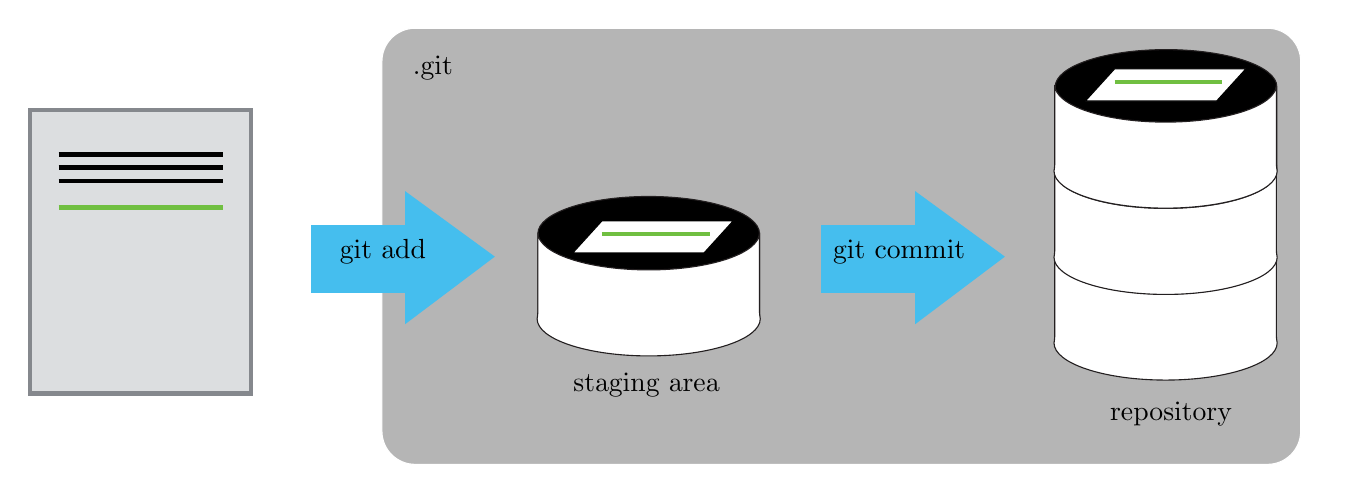
\begin{tikzpicture}[y=0.80pt,x=0.80pt,yscale=-1, inner sep=0pt, outer sep=0pt]
      \path[draw=cFFFFFF,fill=cB5B5B5,miter limit=10.00] (598.0000,23.0000) ..
        controls (598.0000,14.7160) and (591.2840,8.0000) .. (583.0000,8.0000) --
        (198.0000,8.0000) .. controls (189.7160,8.0000) and (183.0000,14.7160) ..
        (183.0000,23.0000) -- (183.0000,190.0000) .. controls (183.0000,198.2840) and
        (189.7160,205.0000) .. (198.0000,205.0000) -- (583.0000,205.0000) .. controls
        (591.2840,205.0000) and (598.0000,198.2840) .. (598.0000,190.0000) --
        (598.0000,23.0000) -- cycle;
      \path[rounded corners=0.0000cm] (197.0000,19.0000) rectangle (267.0000,47.0000);
      \path[cm={{1.0,0.0,0.0,1.0,(197.0,31.4199)}}] (0,0) node[above right] (text9)
        {.git };
        \path[draw=c231F20,fill=black,miter limit=10.00] (253.4530,138.2060) .. controls
          (253.4530,128.9420) and (275.8570,121.4280) .. (303.5000,121.4280) .. controls
          (331.1430,121.4280) and (353.5450,128.9420) .. (353.5450,138.2060) --
          (353.5450,139.2340) .. controls (353.5450,139.2340) and (353.5450,137.1190) ..
          (353.5450,136.1170) .. controls (353.5450,135.1110) and (353.5450,100.3730) ..
          (353.5450,100.3730) -- (353.5450,100.7670) .. controls (353.5450,91.4970) and
          (331.1430,83.9870) .. (303.5000,83.9870) .. controls (275.8570,83.9870) and
          (253.4530,91.4970) .. (253.4530,100.7670) -- (253.4530,100.3730) .. controls
          (253.4530,100.3730) and (253.4530,134.8920) .. (253.4530,136.1060) .. controls
          (253.4530,137.3110) and (253.4530,139.2340) .. (253.4530,139.2340) --
          (253.4530,138.2060) -- cycle;
          \path[draw=c231F20,fill=cFFFFFF,miter limit=10.00] (353.5450,100.3730) ..
            controls (353.5450,100.3730) and (353.5450,135.1110) .. (353.5450,136.1170) ..
            controls (353.5450,137.1190) and (353.9000,139.2340) .. (353.9000,139.2340) ..
            controls (353.9000,148.5050) and (331.1420,156.0140) .. (303.5000,156.0140) ..
            controls (275.8580,156.0140) and (253.1000,148.5050) .. (253.1000,139.2340) ..
            controls (253.1000,139.2340) and (253.4540,137.3110) .. (253.4540,136.1060) ..
            controls (253.4540,134.8920) and (253.4540,100.3730) .. (253.4540,100.3730) ..
            controls (253.4540,109.6470) and (275.8580,117.1580) .. (303.5010,117.1580) ..
            controls (331.1440,117.1580) and (353.5450,109.6470) .. (353.5450,100.3730) --
            cycle;
        \path[draw=black,fill=cFFFFFF,miter limit=10.00] (341.7190,94.9650) --
          (282.4110,94.9650) -- (269.2350,109.4590) -- (328.5420,109.4590) -- cycle;
        \path[draw=c70BF41,line width=1.600pt] (282.4110,100.8940) --
          (331.1650,100.8940);
      \path[draw=c231F20,fill=black,miter limit=10.00] (487.1300,71.8820) .. controls
        (487.1300,62.6140) and (509.5370,55.1010) .. (537.1770,55.1010) .. controls
        (564.8180,55.1010) and (587.2240,62.6140) .. (587.2240,71.8820) --
        (587.2240,72.9120) .. controls (587.2240,72.9120) and (587.2240,70.7940) ..
        (587.2240,69.7910) .. controls (587.2240,68.7880) and (587.2240,34.0520) ..
        (587.2240,34.0520) -- (587.2240,34.4400) .. controls (587.2240,25.1720) and
        (564.8180,17.6590) .. (537.1770,17.6590) .. controls (509.5370,17.6590) and
        (487.1300,25.1720) .. (487.1300,34.4400) -- (487.1300,34.0520) .. controls
        (487.1300,34.0520) and (487.1300,68.5710) .. (487.1300,69.7800) .. controls
        (487.1300,70.9890) and (487.1300,72.9120) .. (487.1300,72.9120) --
        (487.1300,71.8820) -- cycle;
        \path[draw=c231F20,fill=cFFFFFF,miter limit=10.00] (587.0210,111.2840) ..
          controls (587.0210,111.2840) and (587.0210,146.0210) .. (587.0210,147.0230) ..
          controls (587.0210,148.0260) and (587.3750,150.1450) .. (587.3750,150.1450) ..
          controls (587.3750,159.4130) and (564.6150,166.9240) .. (536.9750,166.9240) ..
          controls (509.3350,166.9240) and (486.5760,159.4120) .. (486.5760,150.1450) ..
          controls (486.5760,150.1450) and (486.9290,148.2220) .. (486.9290,147.0130) ..
          controls (486.9290,145.8040) and (486.9290,111.2840) .. (486.9290,111.2840) ..
          controls (486.9290,120.5520) and (509.3360,128.0640) .. (536.9760,128.0640) ..
          controls (564.6140,128.0640) and (587.0210,120.5510) .. (587.0210,111.2840) --
          cycle;
        \path[draw=c231F20,fill=cFFFFFF,miter limit=10.00] (587.0210,72.6010) ..
          controls (587.0210,72.6010) and (587.0210,107.3370) .. (587.0210,108.3400) ..
          controls (587.0210,109.3420) and (587.3750,111.4600) .. (587.3750,111.4600) ..
          controls (587.3750,120.7280) and (564.6150,128.2400) .. (536.9750,128.2400) ..
          controls (509.3350,128.2400) and (486.5760,120.7270) .. (486.5760,111.4600) ..
          controls (486.5760,111.4600) and (486.9290,109.5370) .. (486.9290,108.3280) ..
          controls (486.9290,107.1190) and (486.9290,72.6000) .. (486.9290,72.6000) ..
          controls (486.9290,81.8680) and (509.3360,89.3800) .. (536.9760,89.3800) ..
          controls (564.6140,89.3810) and (587.0210,81.8690) .. (587.0210,72.6010) --
          cycle;
        \path[draw=c231F20,fill=cFFFFFF,miter limit=10.00] (587.0210,33.6280) ..
          controls (587.0210,33.6280) and (587.0210,68.3650) .. (587.0210,69.3670) ..
          controls (587.0210,70.3690) and (587.3750,72.4870) .. (587.3750,72.4870) ..
          controls (587.3750,81.7560) and (564.6150,89.2680) .. (536.9750,89.2680) ..
          controls (509.3350,89.2680) and (486.5760,81.7550) .. (486.5760,72.4870) ..
          controls (486.5760,72.4870) and (486.9290,70.5650) .. (486.9290,69.3560) ..
          controls (486.9290,68.1470) and (486.9290,33.6280) .. (486.9290,33.6280) ..
          controls (486.9290,42.8960) and (509.3360,50.4080) .. (536.9760,50.4080) ..
          controls (564.6140,50.4090) and (587.0210,42.8960) .. (587.0210,33.6280) --
          cycle;
        \path[draw=black,fill=cFFFFFF,miter limit=10.00] (573.2160,26.3810) --
          (513.9080,26.3810) -- (500.7320,40.8750) -- (560.0390,40.8750) -- cycle;
        \path[draw=c70BF41,line width=1.600pt] (513.9080,32.3110) -- (562.6620,32.3110);
        \path[fill=cDCDEE0,rounded corners=0.0000cm] (24.0000,45.0000) rectangle
          (124.0000,173.0000);
        \path[draw=c85888D,line width=1.600pt,rounded corners=0.0000cm]
          (24.0000,45.0000) rectangle (124.0000,173.0000);
        \path[draw=black,line width=1.600pt] (37.0000,65.0000) -- (111.0000,65.0000);
        \path[draw=black,line width=1.600pt] (37.0000,71.0000) -- (111.0000,71.0000);
        \path[draw=black,line width=1.600pt] (37.0000,77.0000) -- (111.0000,77.0000);
        \path[draw=c70BF41,line width=1.600pt] (37.0000,89.0000) -- (111.0000,89.0000);
        \path[fill=c45BEEE,rounded corners=0.0000cm] (150.8710,96.7680) rectangle
          (196.8270,127.3720);
        \path[fill=c45BEEE] (193.4670,81.5710) -- (193.4670,141.6960) --
          (234.0200,111.1630) -- cycle;
      \path[rounded corners=0.0000cm] (164.0000,106.0690) rectangle
        (216.7430,120.0690);
      \path[cm={{1.0,0.0,0.0,1.0,(164.0,114.3496)}}] (0,0) node[above right] (text85)
        {git add };
        \path[fill=c45BEEE,rounded corners=0.0000cm] (381.2510,96.7680) rectangle
          (427.2070,127.3720);
        \path[fill=c45BEEE] (423.8470,81.5710) -- (423.8470,141.6960) --
          (464.3990,111.1630) -- cycle;
      \path[rounded corners=0.0000cm] (376.9800,106.0690) rectangle
        (462.5220,120.0690);
      \path[cm={{1.0,0.0,0.0,1.0,(386.7637,114.3496)}}] (0,0) node[above right]
        (text95) {git commit };
      \path[rounded corners=0.0000cm] (229.0000,166.0000) rectangle
        (376.0000,183.0000);
      \path[cm={{1.0,0.0,0.0,1.0,(269.4766,174.6279)}}] (0,0) node[above right]
        (text99) {staging area };
      \path[rounded corners=0.0000cm] (464.7850,179.0000) rectangle
        (611.7850,196.0000);
      \path[cm={{1.0,0.0,0.0,1.0,(511.9414,187.6279)}}] (0,0) node[above right]
        (text103) {repository };

    \end{tikzpicture}
  \end{minipage}
  }

\end{frame}

\begin{frame}[fragile]
  \frametitle{Tracking changes\footnote{http://swcarpentry.github.io/git-novice/04-changes/}}

Edit the file \texttt{mars.txt} so that it reads (e.g.~using \texttt{nano}):
\begin{minted}{text}
Cold and dry, but everything is my favorite color
The two moons may be a problem for Wolfman
But the Mummy will appreciate the lack of humidity
\end{minted}
\vskip 1 em
\pause

See the differences:
\begin{minted}{shell}
$ git diff
\end{minted}
\vskip 1 em
\pause

Re-stage the file, then look at differences again:
\begin{minted}{shell}
$ git add mars.txt
$ git diff
\end{minted}
\vskip 1 em
\pause

To see the differences, we need the \texttt{--staged} flag:
\begin{minted}{shell}
$ git diff --staged
\end{minted}

\end{frame}

\begin{frame}[fragile]

Commit to the repo:
\begin{minted}{shell}
$ git commit -m "Discuss concerns about Mars' climate for Mummy"
$ git status
$ git log
\end{minted}
\vskip 1 em
\pause

\end{frame}


\begin{frame}[fragile]
  \frametitle{Directories in git\footnote{http://swcarpentry.github.io/git-novice/04-changes/}}

Git does not automatically add directories:
\begin{minted}{shell}
$ mkdir directory
$ git status
\end{minted}
\pause
\vskip 1 em

You have to add it explicitly:
\begin{minted}{shell}
$ git add directory
$ git status
\end{minted}

\end{frame}

\begin{frame}
  \frametitle{Committing\footnote{http://swcarpentry.github.io/git-novice/04-changes/}}

  \resizebox{0.9\textwidth}{!}{
  \begin{minipage}{\textwidth}
    % This was converted from
    % <http://swcarpentry.github.io/git-novice/fig/git-committing.svg>
    % using Inkscape
    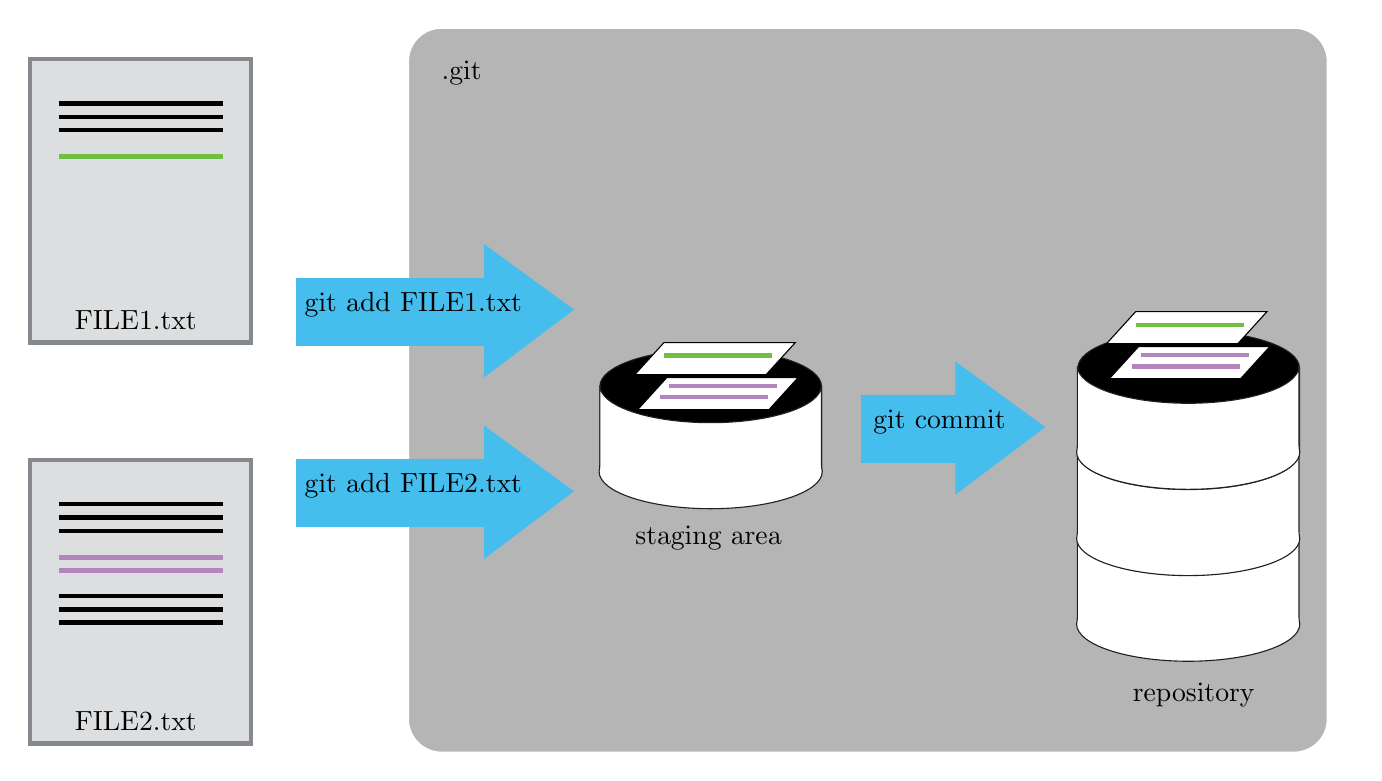
\begin{tikzpicture}[y=0.80pt,x=0.80pt,yscale=-1, inner sep=0pt, outer sep=0pt]
      \path[draw=cFFFFFF,fill=cB5B5B5,miter limit=10.00] (610.0000,23.0000) ..
        controls (610.0000,14.7160) and (603.2840,8.0000) .. (595.0000,8.0000) --
        (210.0000,8.0000) .. controls (201.7160,8.0000) and (195.0000,14.7160) ..
        (195.0000,23.0000) -- (195.0000,320.0000) .. controls (195.0000,328.2840) and
        (201.7160,335.0000) .. (210.0000,335.0000) -- (595.0000,335.0000) .. controls
        (603.2840,335.0000) and (610.0000,328.2840) .. (610.0000,320.0000) --
        (610.0000,23.0000) -- cycle;
      \path[rounded corners=0.0000cm] (210.0000,21.0000) rectangle (280.0000,49.0000);
      \path[cm={{1.0,0.0,0.0,1.0,(210.0,33.4199)}}] (0,0) node[above right] (text9220)
        {.git };
        \path[draw=c231F20,fill=black,miter limit=10.00] (281.4530,207.2190) .. controls
          (281.4530,197.9550) and (303.8570,190.4420) .. (331.5000,190.4420) .. controls
          (359.1430,190.4420) and (381.5450,197.9560) .. (381.5450,207.2190) --
          (381.5450,208.2480) .. controls (381.5450,208.2480) and (381.5450,206.1330) ..
          (381.5450,205.1310) .. controls (381.5450,204.1240) and (381.5450,169.3870) ..
          (381.5450,169.3870) -- (381.5450,169.7800) .. controls (381.5450,160.5100) and
          (359.1430,153.0010) .. (331.5000,153.0010) .. controls (303.8570,153.0010) and
          (281.4530,160.5110) .. (281.4530,169.7800) -- (281.4530,169.3870) .. controls
          (281.4530,169.3870) and (281.4530,203.9060) .. (281.4530,205.1190) .. controls
          (281.4530,206.3240) and (281.4530,208.2480) .. (281.4530,208.2480) --
          (281.4530,207.2190) -- cycle;
          \path[draw=c231F20,fill=cFFFFFF,miter limit=10.00] (381.5450,169.3870) ..
            controls (381.5450,169.3870) and (381.5450,204.1240) .. (381.5450,205.1310) ..
            controls (381.5450,206.1330) and (381.9000,208.2480) .. (381.9000,208.2480) ..
            controls (381.9000,217.5180) and (359.1420,225.0270) .. (331.5000,225.0270) ..
            controls (303.8580,225.0270) and (281.1000,217.5170) .. (281.1000,208.2480) ..
            controls (281.1000,208.2480) and (281.4540,206.3240) .. (281.4540,205.1190) ..
            controls (281.4540,203.9050) and (281.4540,169.3870) .. (281.4540,169.3870) ..
            controls (281.4540,178.6600) and (303.8580,186.1710) .. (331.5010,186.1710) ..
            controls (359.1440,186.1710) and (381.5450,178.6600) .. (381.5450,169.3870) --
            cycle;
        \path[draw=black,fill=cFFFFFF,miter limit=10.00] (369.7190,149.9790) --
          (310.4110,149.9790) -- (297.2350,164.4730) -- (356.5420,164.4730) -- cycle;
        \path[draw=c70BF41,line width=1.600pt] (310.4110,155.9080) --
          (359.1650,155.9080);
        \path[draw=black,fill=cFFFFFF,miter limit=10.00] (371.0290,165.7530) --
          (311.7220,165.7530) -- (298.5460,180.2470) -- (357.8530,180.2470) -- cycle;
        \path[draw=cB285BC,line width=1.600pt] (312.7220,169.6830) --
          (361.4760,169.6830);
        \path[draw=cB285BC,line width=1.600pt] (308.7220,174.6830) --
          (357.4760,174.6830);
      \path[draw=c231F20,fill=black,miter limit=10.00] (497.3450,198.8830) .. controls
        (497.3450,189.6150) and (519.7520,182.1020) .. (547.3920,182.1020) .. controls
        (575.0330,182.1020) and (597.4390,189.6160) .. (597.4390,198.8830) --
        (597.4390,199.9120) .. controls (597.4390,199.9120) and (597.4390,197.7950) ..
        (597.4390,196.7920) .. controls (597.4390,195.7890) and (597.4390,161.0530) ..
        (597.4390,161.0530) -- (597.4390,161.4420) .. controls (597.4390,152.1740) and
        (575.0330,144.6610) .. (547.3920,144.6610) .. controls (519.7520,144.6610) and
        (497.3450,152.1750) .. (497.3450,161.4420) -- (497.3450,161.0530) .. controls
        (497.3450,161.0530) and (497.3450,195.5730) .. (497.3450,196.7820) .. controls
        (497.3450,197.9910) and (497.3450,199.9130) .. (497.3450,199.9130) --
        (497.3450,198.8830) -- cycle;
        \path[draw=c231F20,fill=cFFFFFF,miter limit=10.00] (597.2350,238.2830) ..
          controls (597.2350,238.2830) and (597.2350,273.0210) .. (597.2350,274.0230) ..
          controls (597.2350,275.0250) and (597.5890,277.1440) .. (597.5890,277.1440) ..
          controls (597.5890,286.4120) and (574.8290,293.9230) .. (547.1890,293.9230) ..
          controls (519.5490,293.9230) and (496.7900,286.4110) .. (496.7900,277.1440) ..
          controls (496.7900,277.1440) and (497.1430,275.2200) .. (497.1430,274.0110) ..
          controls (497.1430,272.8020) and (497.1430,238.2820) .. (497.1430,238.2820) ..
          controls (497.1430,247.5500) and (519.5500,255.0630) .. (547.1900,255.0630) ..
          controls (574.8290,255.0640) and (597.2350,247.5510) .. (597.2350,238.2830) --
          cycle;
        \path[draw=c231F20,fill=cFFFFFF,miter limit=10.00] (597.2350,199.6020) ..
          controls (597.2350,199.6020) and (597.2350,234.3380) .. (597.2350,235.3400) ..
          controls (597.2350,236.3420) and (597.5890,238.4610) .. (597.5890,238.4610) ..
          controls (597.5890,247.7290) and (574.8290,255.2400) .. (547.1890,255.2400) ..
          controls (519.5490,255.2400) and (496.7900,247.7280) .. (496.7900,238.4610) ..
          controls (496.7900,238.4610) and (497.1430,236.5370) .. (497.1430,235.3280) ..
          controls (497.1430,234.1190) and (497.1430,199.6010) .. (497.1430,199.6010) ..
          controls (497.1430,208.8690) and (519.5500,216.3800) .. (547.1900,216.3800) ..
          controls (574.8290,216.3810) and (597.2350,208.8690) .. (597.2350,199.6020) --
          cycle;
        \path[draw=c231F20,fill=cFFFFFF,miter limit=10.00] (597.2350,160.6290) ..
          controls (597.2350,160.6290) and (597.2350,195.3650) .. (597.2350,196.3670) ..
          controls (597.2350,197.3700) and (597.5890,199.4880) .. (597.5890,199.4880) ..
          controls (597.5890,208.7560) and (574.8290,216.2690) .. (547.1890,216.2690) ..
          controls (519.5490,216.2690) and (496.7900,208.7550) .. (496.7900,199.4880) ..
          controls (496.7900,199.4880) and (497.1430,197.5650) .. (497.1430,196.3560) ..
          controls (497.1430,195.1470) and (497.1430,160.6280) .. (497.1430,160.6280) ..
          controls (497.1430,169.8960) and (519.5500,177.4070) .. (547.1900,177.4070) ..
          controls (574.8290,177.4080) and (597.2350,169.8960) .. (597.2350,160.6290) --
          cycle;
        \path[draw=black,fill=cFFFFFF,miter limit=10.00] (584.0860,151.7740) --
          (524.7780,151.7740) -- (511.6030,166.2690) -- (570.9090,166.2690) -- cycle;
        \path[draw=cB285BC,line width=1.600pt] (525.7780,155.7040) --
          (574.5320,155.7040);
        \path[draw=cB285BC,line width=1.600pt] (521.7780,160.7040) --
          (570.5320,160.7040);
        \path[draw=black,fill=cFFFFFF,miter limit=10.00] (582.7750,136.0000) --
          (523.4680,136.0000) -- (510.2920,150.4940) -- (569.5990,150.4940) -- cycle;
        \path[draw=c70BF41,line width=1.600pt] (523.4680,141.9300) --
          (572.2220,141.9300);
        \path[fill=cDCDEE0,rounded corners=0.0000cm] (24.0000,22.0000) rectangle
          (124.0000,150.0000);
        \path[draw=c85888D,line width=1.600pt,rounded corners=0.0000cm]
          (24.0000,22.0000) rectangle (124.0000,150.0000);
        \path[draw=black,line width=1.600pt] (37.0000,42.0000) -- (111.0000,42.0000);
        \path[draw=black,line width=1.600pt] (37.0000,48.0000) -- (111.0000,48.0000);
        \path[draw=black,line width=1.600pt] (37.0000,54.0000) -- (111.0000,54.0000);
        \path[draw=c70BF41,line width=1.600pt] (37.0000,66.0000) -- (111.0000,66.0000);
      \path[rounded corners=0.0000cm] (27.6280,136.0000) rectangle
        (120.3710,150.0000);
      \path[cm={{1.0,0.0,0.0,1.0,(44.3105,144.2803)}}] (0,0) node[above right]
        (text9305) {FILE1.txt };
        \path[fill=cDCDEE0,rounded corners=0.0000cm] (24.0000,203.0000) rectangle
          (124.0000,331.0000);
        \path[draw=c85888D,line width=1.600pt,rounded corners=0.0000cm]
          (24.0000,203.0000) rectangle (124.0000,331.0000);
        \path[draw=black,line width=1.600pt] (37.0000,223.0000) -- (111.0000,223.0000);
        \path[draw=black,line width=1.600pt] (37.0000,229.0000) -- (111.0000,229.0000);
        \path[draw=black,line width=1.600pt] (37.0000,235.0000) -- (111.0000,235.0000);
        \path[draw=black,line width=1.600pt] (37.0000,264.5140) -- (111.0000,264.5140);
        \path[draw=black,line width=1.600pt] (37.0000,270.5140) -- (111.0000,270.5140);
        \path[draw=black,line width=1.600pt] (37.0000,276.5140) -- (111.0000,276.5140);
        \path[draw=cB285BC,line width=1.600pt] (37.0000,247.0000) --
          (111.0000,247.0000);
        \path[draw=cB285BC,line width=1.600pt] (37.0000,253.0000) --
          (111.0000,253.0000);
        \path[rounded corners=0.0000cm] (27.6280,317.0000) rectangle
          (120.3710,331.0000);
        \path[cm={{1.0,0.0,0.0,1.0,(44.3105,325.2803)}}] (0,0) node[above right]
          (text9331) {FILE2.txt };
    \path[rounded corners=0.0000cm] (395.1950,183.0690) rectangle
      (480.7370,197.0690);
        \path[fill=c45beee,rounded corners=0.0000cm] (399.4660,173.7680) rectangle
          (445.4220,204.3720);
        \path[fill=c45beee] (482.6140,188.1630) -- (442.0620,158.5710) --
          (442.0620,218.6950) -- cycle;
      \path (404.97849,191.34959) node[above right] (text9366) {git commit };
    \path[rounded corners=0.0000cm] (257.0000,235.0140) rectangle
      (404.0000,252.0140);
    \path (297.47659,243.6416) node[above right] (text9370) {staging area };
    \path[rounded corners=0.0000cm] (475.0000,306.0000) rectangle
      (622.0000,323.0000);
    \path (522.15619,314.6279) node[above right] (text9374) {repository };
      \begin{scope}[shift={(-212.84669,28.971837)}]
        \path[fill=c45beee,rounded corners=0.0000cm] (356.8467,173.7680) rectangle
          (445.4220,204.3720);
        \path[fill=c45beee] (442.0620,218.6950) -- (482.6140,188.1630) --
          (442.0620,158.5710) -- cycle;
      \end{scope}
      \path (148.13179,220.32143) node[above right] (text9417) {git add FILE2.txt };
    \begin{scope}[shift={(0,-82.0)}]
      \begin{scope}[shift={(-212.84669,28.971837)}]
        \path[fill=c45beee,rounded corners=0.0000cm] (356.8467,173.7680) rectangle
          (445.4220,204.3720);
        \path[fill=c45beee] (442.0620,158.5710) -- (442.0620,218.6950) --
          (482.6140,188.1630) -- cycle;
      \end{scope}
      \path (148.13179,220.32143) node[above right] (text9451) {git add FILE1.txt };
    \end{scope}

    \end{tikzpicture}

  \end{minipage}
}
\end{frame}

\begin{frame}[fragile]
\frametitle{Exercise: Choosing a Commit Message\footnote{\url{http://swcarpentry.github.io/git-novice/04-changes/\#choosing-a-commit-message}}}

Which of the following commit messages would be most appropriate for the last commit made to \texttt{mars.txt}?

\begin{enumerate}
  \item ``Changes'' \onslide<2->{\wrongans}
  \item ``Added line 'But the Mummy will appreciate the lack of humidity' to mars.txt'' \onslide<2->{\wrongans}
  \item ``Discuss effects of Mars’ climate on the Mummy'' \onslide<2->{\correctans}
\end{enumerate}

\vskip 1 em
\onslide<3->{Answer 1 is not descriptive enough, and answer 2 is too descriptive and redundant, but answer 3 is good: short but descriptive.}


\end{frame}

\begin{frame}
% Blank frame
\end{frame}

\begin{frame}
\frametitle{Copyright notice}

The materials here are based on the lesson plans provided by Software Carpentry at \url{http://swcarpentry.github.io/git-novice/}, and are used under the Creative Commons Attribution 4.0 license (\url{https://software-carpentry.org/license/}).

\vskip 3 em

These materials are available under the Creative Commons Attribution 4.0 license (\url{https://software-carpentry.org/license/}).

\end{frame}

\end{document}
